%\documentclass[handout,xcolor=pdftex,dvipsnames,table]{beamer}
%\documentclass[draft]{beamer}
%\documentclass[notesonly]{beamer}
%\documentclass[notes]{beamer}
\documentclass[aspectratio=169, xcolor=table]{beamer}\usepackage[]{graphicx}\usepackage[]{color}
%% maxwidth is the original width if it is less than linewidth
%% otherwise use linewidth (to make sure the graphics do not exceed the margin)
\makeatletter
\def\maxwidth{ %
  \ifdim\Gin@nat@width>\linewidth
    \linewidth
  \else
    \Gin@nat@width
  \fi
}
\makeatother

\definecolor{fgcolor}{rgb}{0.345, 0.345, 0.345}
\newcommand{\hlnum}[1]{\textcolor[rgb]{0.686,0.059,0.569}{#1}}%
\newcommand{\hlstr}[1]{\textcolor[rgb]{0.192,0.494,0.8}{#1}}%
\newcommand{\hlcom}[1]{\textcolor[rgb]{0.678,0.584,0.686}{\textit{#1}}}%
\newcommand{\hlopt}[1]{\textcolor[rgb]{0,0,0}{#1}}%
\newcommand{\hlstd}[1]{\textcolor[rgb]{0.345,0.345,0.345}{#1}}%
\newcommand{\hlkwa}[1]{\textcolor[rgb]{0.161,0.373,0.58}{\textbf{#1}}}%
\newcommand{\hlkwb}[1]{\textcolor[rgb]{0.69,0.353,0.396}{#1}}%
\newcommand{\hlkwc}[1]{\textcolor[rgb]{0.333,0.667,0.333}{#1}}%
\newcommand{\hlkwd}[1]{\textcolor[rgb]{0.737,0.353,0.396}{\textbf{#1}}}%
\let\hlipl\hlkwb

\usepackage{framed}
\makeatletter
\newenvironment{kframe}{%
 \def\at@end@of@kframe{}%
 \ifinner\ifhmode%
  \def\at@end@of@kframe{\end{minipage}}%
  \begin{minipage}{\columnwidth}%
 \fi\fi%
 \def\FrameCommand##1{\hskip\@totalleftmargin \hskip-\fboxsep
 \colorbox{shadecolor}{##1}\hskip-\fboxsep
     % There is no \\@totalrightmargin, so:
     \hskip-\linewidth \hskip-\@totalleftmargin \hskip\columnwidth}%
 \MakeFramed {\advance\hsize-\width
   \@totalleftmargin\z@ \linewidth\hsize
   \@setminipage}}%
 {\par\unskip\endMakeFramed%
 \at@end@of@kframe}
\makeatother

\definecolor{shadecolor}{rgb}{.97, .97, .97}
\definecolor{messagecolor}{rgb}{0, 0, 0}
\definecolor{warningcolor}{rgb}{1, 0, 1}
\definecolor{errorcolor}{rgb}{1, 0, 0}
\newenvironment{knitrout}{}{} % an empty environment to be redefined in TeX

\usepackage{alltt}  % xcolor to avoid conflict
                                                       %  with beamer
\mode<presentation>
% https://hartwork.org/beamer-theme-matrix/
\usetheme{Singapore} %Berkeley, Palo Alto, Singapore, Warsaw
\usecolortheme{seahorse}  %Beaver, dolphin, dove, lily, orchid, seagull, seahorse
\renewcommand{\insertnavigation}[1]{}    % to remove contents bar:
           % https://tex.stackexchange.com/questions/33767/remove-section-header-from-a-beamer-theme-singapore

%\usefonttheme{serif}
% font themes: default, professionalfonts, serif, structurebold, structureitalicserif, structuresmallcapsserif

\usepackage{graphicx}
\usepackage{pgf}
\usepackage{array}
\usepackage{tabularx}
\usepackage{multicol}          %% Multiple columns for itemize
%\usepackage{booktabs}          %% Used in risk tables [hake]
%\usepackage{multirow}          %% Used in decision tables [hake]
%\usepackage{beamerarticle}
%\usepackage{enumitem}
%\usepackage{beamerthemesplit}
\usepackage[T1]{fontenc}  %to use < or > in tables
% \usepackage{xcolor}            %% for kable
% \usepackage[table]{xcolor}            %% for kable

% From kableExtra documentation, commenting out some:
\usepackage{longtable}
\usepackage{array}
\usepackage[table]{xcolor}
\usepackage{booktabs}          %% Used in risk tables [hake]
\usepackage{multirow}          %% Used in decision tables [hake]

\usepackage{wrapfig}
\usepackage{float}
\usepackage{colortbl}
\usepackage{pdflscape}
\usepackage{tabu}
\usepackage{threeparttable}
\usepackage{threeparttablex}
\usepackage[normalem]{ulem}
\usepackage{makecell}

\usepackage[export]{adjustbox}     % for left and right in \includegraphics
\usepackage[absolute,overlay]{textpos}  % for overlaying text

\newcolumntype{Y}{>{\centering\arraybackslash}X}
%% syntax is \mlc{first line\\secondline}
\newcommand{\mlc}[2][c]{\begin{tabular}[#1]{@{}c@{}}#2\end{tabular}}
\newcommand{\subscr}[1]{$_{\text{#1}}$}\newcommand{\Fforty}{F_{\text{SPR}=40\%}}       % Needs to be done as $\Fforty$
\newcommand{\Bforty}{B_{\text{SPR}=40\%}}

% pdf is displayed in full screen mode automatically
%\hypersetup{pdfpagemode=FullScreen}

%\setbeamersize{sidebar width left=0.05in}
\setbeamersize{text margin left=5mm}
\setbeamersize{text margin right=5mm}

\setbeamertemplate{title page}
{
% Looks like for hake we didn't use the defaults and played with the spacing
% \vskip0pt plus 1filll
\begin{center}
\vskip6pt
{\usebeamerfont{title}\usebeamercolor[fg]{title}\inserttitle}\\
\vskip22pt
\insertauthor
\vskip22pt
\insertinstitute
% \insertdate
\end{center}
% \vskip30pt
\vfill
\usebeamerfont{subtitle}\usebeamercolor[fg]{subtitle}\insertsubtitle % \par
% \vskip0pt plus 1filll
\hfill

\includegraphics[width=4.8cm]{images/DFO_Logo.png}   % from Wikipedia (for hake we
% had an older one)
\includegraphics[width=1cm]{images/UBC-logo.jpg}
\vskip10pt
}

\definecolor{pageCol}{rgb}{0.5,0.5,1.0}

\setbeamertemplate{footline}
{
\begin{beamercolorbox}[wd=.05\paperwidth,ht=0ex,dp=0ex,left]{framenumber in head/foot}%
\insertframenumber/\inserttotalframenumber
\end{beamercolorbox}%
}
%% \setbeamercolor{footline}{fg=pageCol}

\newcounter{saveenumi}

\newcommand{\blue}{\textcolor{blue}}
\newcommand{\red}{\textcolor{red}}
\newcommand{\bc}{\begin{center}}
\newcommand{\ec}{\end{center}}
\newcommand{\bn}{\begin{enumerate}}
\newcommand{\en}{\end{enumerate}}
\newcommand{\bi}{\begin{itemize}}
\newcommand{\ei}{\end{itemize}}
\newcommand{\Bmsy}{B_{\mbox{\tiny{MSY}}}}
\newcommand{\howlikely}{How likely are different values of $p$ (the underlying probability of getting a head)?}
%% <<echo=TRUE,  message=TRUE, results='show', warning=TRUE>>=
%% opts_chunk$set(dev='cairo_ps',fig.path='knitr-cache/', fig.dpi=96, fig.width=7.5,
%%                fig.height=4, echo=TRUE, results=TRUE, message=TRUE, warning=TRUE,
%%                results='show', cache=TRUE, cache.path='knitr-cache/')


%%%%%%%%%%%%%%%%%%%%%%%%%%%%%%%%%%%%%%%%%%%%%%%%%%%%%%%%%%%%%%%%%


% See https://github.com/pbs-assess/TESA-uncertainty-talk for formatting examples

\title[Notation]{~\\ Some guidance on using mathematical notation in biology}
\author{Andrew Edwards$^1$ \& Marie Auger-M\'eth\'e$^2$
  \\ ~\\ 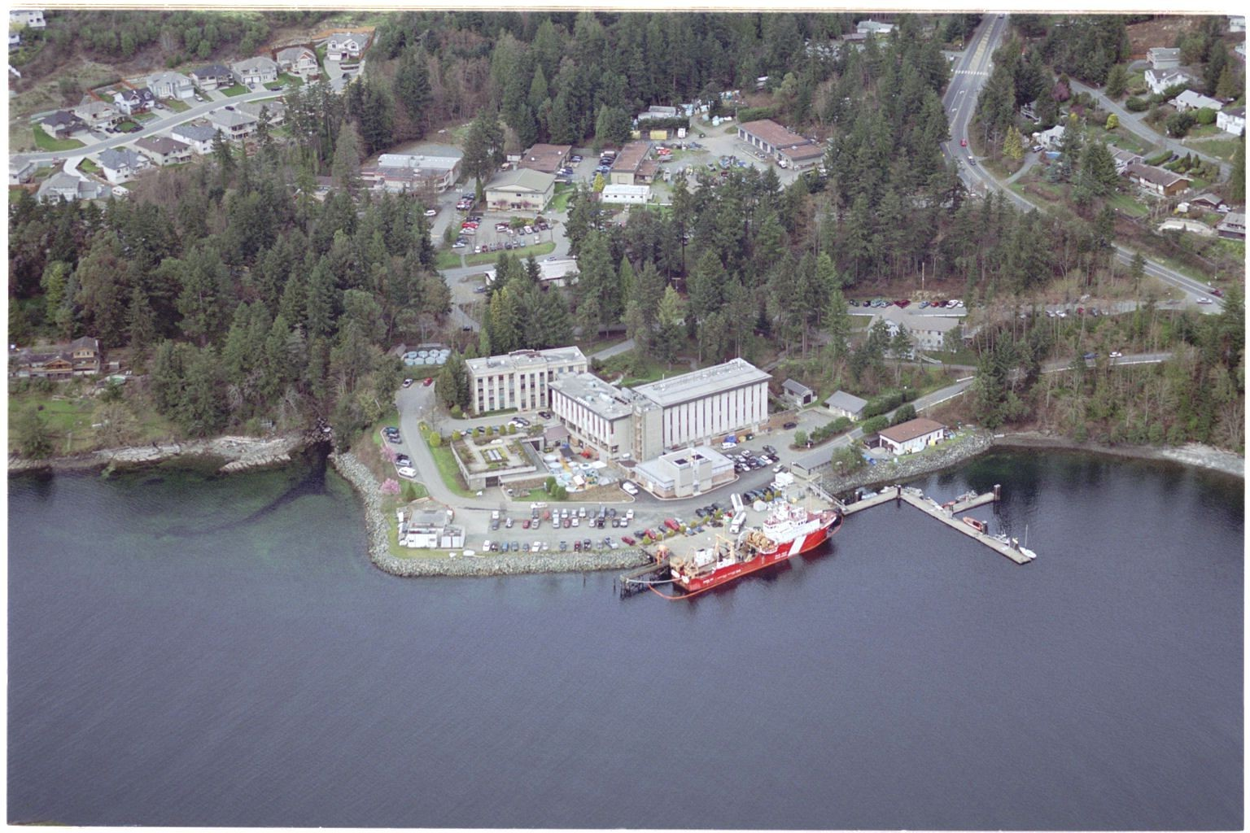
\includegraphics[height=3.5cm]{images/pbs.png}\\
  ~\\ \textcolor{blue}{$^1$Pacific Biological Station \& University of Victoria;
  $^2$University of British Columbia}}
% \institute{{\textcolor{blue}{Pacific Biological Station, Nanaimo, BC}\\
%  ~\\
% \institute{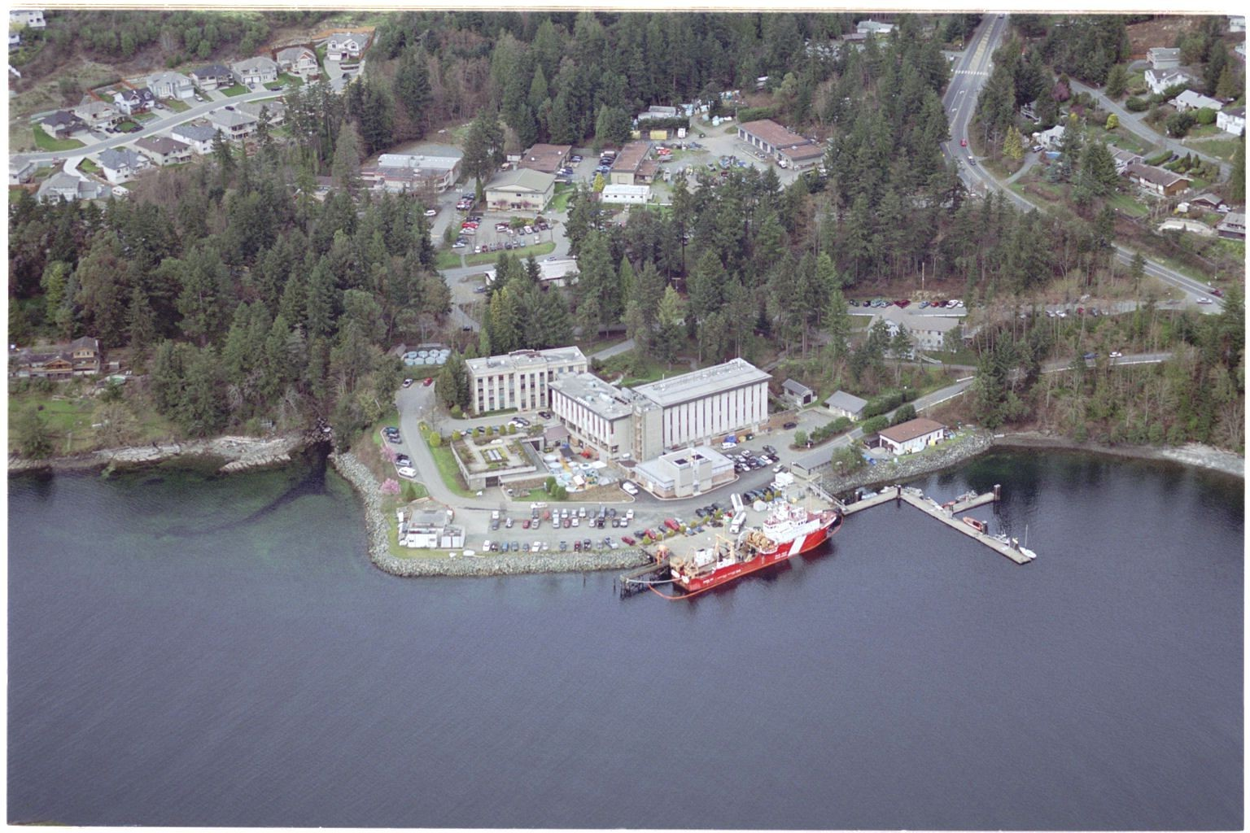
\includegraphics[height=3cm]{images/pbs.png}}
% \titlegraphic{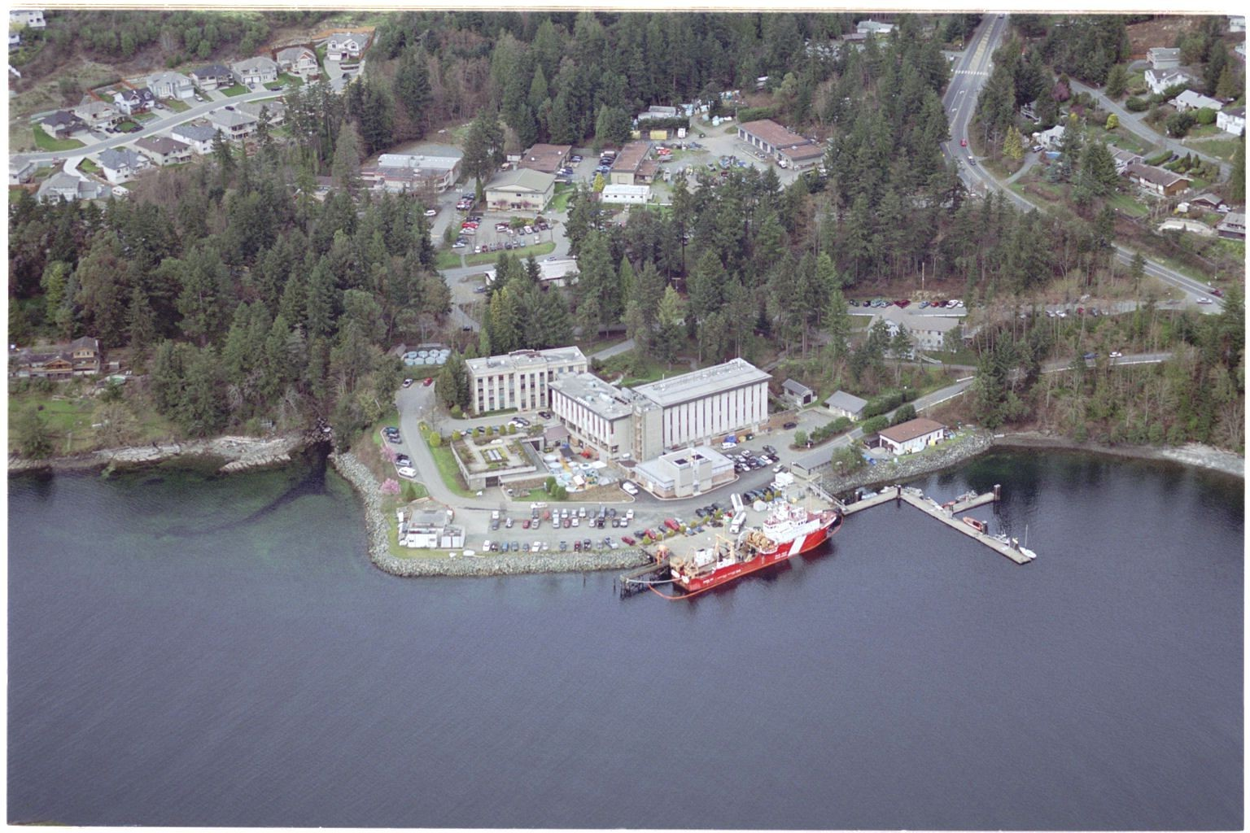
\includegraphics[height=3.3cm]{images/pbs.png}}
% \titlegraphic{images/pbs.png}
\date{{\footnotesize SRG meeting -- 2018}}
\subtitle{\small UVic Biology Department Seminar TODO: add UBC photo, tidy up\\
Friday 1st November, 2019}
\IfFileExists{upquote.sty}{\usepackage{upquote}}{}

\setbeamertemplate{background}
{
\includegraphics[width=\paperwidth,height=\paperheight,keepaspectratio]{images/background-trans.png}}

\setbeamertemplate{itemize items}{
\includegraphics[scale=0.017]{images/halloween_pumpkin3.png}}
\setbeamertemplate{itemize subitem}{
\includegraphics[scale=0.017]{images/halloween_pumpkin2.png}}
\setbeamertemplate{itemize subsubitem}{
\includegraphics[scale=0.017]{images/halloween_pumpkin5.png}}

\newcommand{\eb}{\begin{eqnarray}}
\newcommand{\ee}{\end{eqnarray}}

\usefonttheme{serif}
\usepackage{mathptmx}    % Should have Times plus math fonts. AME used for Hake.

\begin{document}

\beamertemplatenavigationsymbolsempty   % bottom navigation panel
% \setbeamertemplate{headline}{}
% \setbeamertemplate{mini frames}{}

%\begin[plain]{frame}
\frame[plain]{
\titlepage
}
%----------------------------------------------------------

\setbeamertemplate{background}
{
\includegraphics[width=\paperwidth,height=\paperheight,keepaspectratio]{images/background-trans2.png}}
% fainter halloween picture for background

%----------------------------------------------------------

%%%%%%%%%%%%%%%%%%%%%%%
%\section{Outline}
%\subsection{}

\begin{frame}
\frametitle{Outline}
\bi
  \item motivation
%  \item \blue{background}
  \item twelve guidelines
  \item \blue{common usage of particular letters \& symbols}
  \item example of confusing notation
  \item \blue{take-home message}
\ei
\end{frame}

%----------------------------------------------------------

\begin{frame}
\frametitle{Motivation}
\bi
\item mathematical modelling playing an increasing role in biology
\item \blue{requires communication of details of models}
\item this includes notation
\item \blue{clarity of notation varies between papers}
\item poor notation can:
  \bi
  \item \red{make models appear more complicated than necessary}
  \item \red{this leads to cluttered equations that impede understanding}
  \item \red{impedes communication of ideas}
  \item \red{can prevent work being properly reviewed -- analogous to an
      incomplete description of the methods of a laboratory experiment}
  \ei
\ei
\end{frame}

%----------------------------------------------------------

\begin{frame}
\frametitle{Why us?}
Make into a table with photos....

Both reviewed manuscripts in which the unclear
notation made it impossible for us to understand the modelling details, and
therefore we could not evaluate the results or conclusions.

Similarities in backgrounds: all research highly quantitiatve
(lead authors of over 20 ecological modelling papers),
Furthermore, we have both taught modelling courses to biology students.

Differences: one undergrad in math, one biology

We ourselves have papers with notation that could, in hindsight, be improved.

Include link to paper

Include link to GitHub repo.
\end{frame}


% ----------------------------------------------------------

\begin{frame}
\frametitle{Motivation}
Lowry (1959) -- increase ``use of mathematical notation
where appropriate in ecological literature''.

TODO: figure:

equations in:
 14\% of the 37~contributions in the issue of \emph{Ecology} containing the
 Lowry (1959)

38\% of the 26~contributions comprising the March 2018 issue.
56\% of the 34~contributions in the March 2018 issue of \emph{Methods in Ecology and Evolution},

Lowry said advantages include:
\bi
\item precise communication of logical thought (beyond that afforded by
  the written word)
\item reproducibility of methods and results
\ei
and they ``accrue in proportion to
\red{the care used by the author in the use of notation}''.
\end{frame}

%----------------------------------------------------------

\begin{frame}
\frametitle{Motivation}
Many skills involved in producing ecological modelling paper, with books covering:
\bi
\item introductory ecology
\item general mathematics
\item ecological modelling
\item implementing models in R
\item writing and publishing a paper
\ei
  Recommendations exist for:
\bi
\item streamlining workflows (tools such as Git and GitHub)
\item making computer code available and reproducible
\ei
But no tips on developing the mathematical notation to use in a model.

\end{frame}

%----------------------------------------------------------

\begin{frame}
\frametitle{Motivation}

Improvements have impacts -- for Individual Based Models:

\bi
\item previously criticised as generally being so poorly documented
that they could not be evaluated or reproduced
\item motivated development of standardised protocols
\item led to a more rigorous formulation of models
\item enhanced understanding
\ei
\end{frame}

%----------------------------------------------------------

\begin{frame}
\frametitle{What is notation?}

\red{notation} -- we are specifically referring to:
\bi
\item letters used to represent quantities in equations
\item use of subscripts, superscripts and related concepts
\ei

Letters are usually taken from the Roman ($a, b, c, ...$) or
Greek ($\alpha, \beta, \gamma, ...$) alphabets, and can be lower or upper case.
\end{frame}

%----------------------------------------------------------

\begin{frame}
\frametitle{What do journals say?}
We reviewed the Author Guidelines for a sample of 14 journals:
\begin{multicols}{2}
\bi
\item \emph{Bulletin of Mathematical Biology}
\item \emph{Canadian Journal of Fisheries and Aquatic Sciences}
\item \emph{Ecology}
\item \emph{Ecology Letters}
\item \emph{Evolution$^*$}
\item \emph{Functional Ecology}
\item \emph{Journal of Animal Ecology}
\item \emph{Journal of the Royal Society Interface$^*$}
\item \emph{Marine Ecology Progress Series}
\item \emph{Methods in Ecology and Evolution}
\item \emph{Molecular Biology and Evolution}
\item \emph{Nature}
\item \emph{PLOS ONE}
\item \emph{Science}
\item[\vspace{\fill}]
\ei
\end{multicols}

$^*$Only two that have no no mention of equations.

Minimal guidance in others -- almost exclusively restricted to typesetting aspects
(such as bold for vectors).

% rather than the broader considerations that we
%present here.
\end{frame}
%----------------------------------------------------------

\begin{frame}
\frametitle{Authors' responsibility}
Onus for good notation should be on authors (rather than journals)
because:
\bi
  \item notation should be decided early on in a study (possibly before deciding on a
    particular journal)
  \item ideally computer code will match the notation
  \item  work may first appear in a technical document such as a thesis before being
      submitted to a journal
  \item Supporting Information of a paper often contains the full mathematical details of
models and is not typeset or edited by publishers -- authors are responsibile for
clarity
\ei
\end{frame}

%----------------------------------------------------------

\begin{frame}
\frametitle{Guidelines}
\bi
  \item based on those traditionally used in mathematics and are in a somewhat
    logical order
  \item our aim is for them to be useful and adopted
  \item though we anticipate exceptions for which they are purposefully
    overlooked
  \item use examples from common ecological models, our own fields of research and from evolutionary biology.
\ei
\end{frame}

%----------------------------------------------------------

\begin{frame}
\frametitle{1. Define all terms}

Who recognises this equation?
\eb
\nonumber E = mc^2
\ee

\pause Who knows what it means?

\medskip

\pause It does not convey any information, since the \red{letters are not
defined}.

\end{frame}

%----------------------------------------------------------

\begin{frame}
\frametitle{1. Define all terms}
Common ecological example:
\eb
\nonumber S = cA^z
\ee
\pause
where:
\bi
\item $S$ represents the number of species (of a particular taxonomic category)
in area $A$
\item constant $c$ is the
  number of species that would be in one square unit
\item dimensionless exponent $z$ quantifies the change in species number with area
\ei

\pause
So equation represents an increase in species richness with area.

\pause

Immediately after an equation (as part of the same sentence)
any previously undefined symbols should be defined using the phrase
\red{``where ...''}.
\end{frame}

%----------------------------------------------------------

\begin{frame}
\frametitle{1. Define all terms}

The number one guideline is to \red{define every term that is used in an equation}.

\pause

The number one guideline is to \red{define every term that is used in an equation}.

\pause

The number one guideline is to \red{define every term that is used in an equation}.

\pause

The number one guideline is to \red{define every term that is used in an equation}.

\pause

\medskip

Maybe introduce a second time if appears again much later in a lengthy work.

\medskip

\red{Table of notation} helpful for for complicated models. TODO example

\medskip

\pause

Desirable for tables and figures to be understandable on their own, so any
notation in them should be
additionally defined in their captions.


\end{frame}

%----------------------------------------------------------

% Sans serif fonts (like Arial) aren't great for math.

\begin{frame}
\frametitle{2. Use italics, boldface and capitalisation appropriately}

By convention, mathematical symbols (except Greek letters) should be italicised.

Distinguishes text from mathematical notation:

\bi
\item a large value of $a$
\item a large value of a [much clearer in a serif font]
\ei

Vectors and matrices should be Roman script and bold:
\bi
\item {\bf a} is a vector
\item {\bf A} is a matrix
\item element $i$ of {\bf a} is often $a_i$
\item element in row $i$ and column $j$ of {\bf A} is  $A_{ij}$ (or sometimes
  $a_{ij}$)
\ei


Generic random variables are usually upper case:  $X$.

Possible numeric values represented by the corresponding lower-case letter: $x$.
\end{frame}

%----------------------------------------------------------


\begin{frame}
\frametitle{2. Use italics, boldface and capitalisation appropriately}

Roman letters for standard mathematical functions:
\bi
\item $\sin x$, $\cos x$, $\log x$, $\ln x$, e$^x$
\ei
and for other words such as:
\eb
\nonumber X \sim \mbox{Normal}(\mu, \sigma^2)
\label{Xnormal}
\ee
\pause
for variable $X$ coming from a normal distribution with mean $\mu$ and
standard deviation $\sigma$.
\pause

\medskip
Also use a Roman d for derivative and integral of variable $X$ with respect to time $t$:
\eb
\nonumber \frac{\mbox{d}X}{\mbox{d}t} ~~~~~~\mbox{and}~~~~~~ \int f(x) \mbox{d}x
\ee

\pause
\medskip

Units should be given in Roman type to distinguish them from mathematical variables:
\bi
\item the speed of the polar bear was 1~km~h$^{-1}$
\item let the speed be $x$~km~h$^{-1}$
\ei

\end{frame}

%----------------------------------------------------------

\begin{frame}
\frametitle{3. Use subscripts appropriately}

Subscripts represent different values of a quantity.

\bi
\item $B_t$ -- biomass of a population in year $t$, where
$t=1, 2, 3, ..., T$, and $T$ is the maximum year.
\ei

\pause

\red{Cannot} then use:

\bi
\item $B_s$ -- biomass in spatial area $s$, where $s=1, 2, 3, ..., S$, and $S$
  is the number of areas.
  \ei

\pause

Because:

\bi
\item $t=1$ gives $B_1$ as the biomass in year 1

\item $s=1$ also gives $B_1$ as the biomass in spatial area 1
\ei

Obvious confusion.

\end{frame}

%----------------------------------------------------------

\begin{frame}
\frametitle{}
\bi
  \item
\ei
\end{frame}

%----------------------------------------------------------

\begin{frame}
\frametitle{}
\bi
  \item
\ei
\end{frame}

%----------------------------------------------------------

\begin{frame}
\frametitle{}
\bi
  \item
\ei
\end{frame}

%----------------------------------------------------------

\begin{frame}
\frametitle{}
\bi
  \item
\ei
\end{frame}

%----------------------------------------------------------

\begin{frame}
\frametitle{}
\bi
  \item
\ei
\end{frame}

%----------------------------------------------------------

\begin{frame}
\frametitle{}
\bi
  \item
\ei
\end{frame}

%----------------------------------------------------------

\begin{frame}
\frametitle{}
\bi
  \item
\ei
\end{frame}

%----------------------------------------------------------

\begin{frame}
\frametitle{}
\bi
  \item
\ei
\end{frame}

%----------------------------------------------------------

\begin{frame}
\frametitle{}
\bi
  \item
\ei
\end{frame}

%----------------------------------------------------------

\begin{frame}
\frametitle{}
\bi
  \item
\ei
\end{frame}

%----------------------------------------------------------

\begin{frame}
\frametitle{}
\bi
  \item
\ei
\end{frame}

%----------------------------------------------------------




\end{document}

Proofreading - mention KH paper


% notation-rev.tex: take some bits to put into talk, delete un-needed:



\section*{Guidelines}


\subsection*{Use italics, boldface and capitalisation appropriately}



\subsection*{Use subscripts appropriately}

In practice there may be interest in modelling the biomass in
area $s$ in year $t$ (for various combinations of $s$ and $t$),
in which case two subscripts are needed: $B_{st}$.
Extending this idea, \citet{ffrr12} analysed data from fish trawl surveys
and defined
$B_{ijkmn}$ as the biomass caught per hour (g~h$^{-1}$) of
taxonomic group $i$,
length class $j$
and haul $k$ by
vessel $m$ in
year $n$. This notation succinctly describes the detailed structure of the data
and makes Fung $et~al.$'s subsequent calculations clear and unambiguous.
For brevity, there may be no need for a comma ($B_{s,t}$) until numbers are
inserted and there
could be ambiguity ($B_{3,17}$ rather than $B_{317}$),
although this can be a matter of personal preference, and we ourselves have
differing inclinations.

An abbreviation can be used as a (non-italicised) subscript to indicate related
definitions.
For example, \citet{olajos18} used $P_\mathrm{fp}$ and $P_\mathrm{fn}$ to
represent the respective probabilities of false positives and false negatives
when modelling DNA records from sediments to study processes such as
evolutionary divergence.
Similarly, $B_\mathrm{MSY}$ is often
used in fisheries to represent the biomass of a stock at the maximum sustainable
yield (MSY). So MSY is being used not as an index (like in $B_t$ above), but as
a non-italicised acronym to
distinguish $B_\mathrm{MSY}$ from the related $B_t$.
Just avoid trying to use $MSY$ alone as
a variable (see below) -- if $Y_t$ represents the yield in
year $t$, then
$Y_\mathrm{MSY}$  would be notationally consistent with
$B_\mathrm{MSY}$.

Usually, a subscript that is used as an index should appear on both sides of
an equation, such as in
\eb
y_t = 2 x_t + 3,
\label{ytxt}
\ee
for the relationship between two variables $x_t$ and $y_t$ at each time $t$ --
there is a value of $y_t$ corresponding to each setting of $t$.

There should generally not be a mixture of subscripts, such as
\eb
y_t = 2 x_i + 3.
\ee
This equation implies that $y_t$ depends on the value of $x_i$, and therefore
on $i$, and so $y_t$ should really be denoted $y_{it}$. Otherwise, for example,
we may have $y_t = 9$
for $x_1 = 3$ (with $i=1$), but $y_t = 13$ for $x_2 = 5$ (with $i=2$) -- but the
notation $y_t$ does not distinguish between the different values for $i=1$ and
$i=2$.

An expression such as
\eb
y_{ij} = 2 x_i + 3
\ee
is valid -- it just means that the $ij$ value of $y$ is the same
for all values of the index $j$ (since nothing on the right-hand side depends
on $j$).

One source of confusion is having $i$ and $j$ as indices, but then using these
again in a summation to sum $N$ values:
\eb
y_{ij} = 2 x_{ij} + \sum_{i=1}^N x_{ij}.
\ee
The problem is that $i$ is used here as an index, such that the equation is
valid for all values of $i$, but then is also used in the summation where it
is just a dummy index. A better formulation would be
\eb
y_{ij} = 2 x_{ij} + \sum_{k=1}^N x_{kj}
\label{sumk}
\ee
where $k$ is a dummy index.
Another way to understand this is to realise that
the following are all equivalent:
\eb
\sum_{k=1}^N x_{kj} = \sum_{l=1}^N x_{lj} = \sum_{m=1}^N x_{mj},
\ee
because $k, l$ and $m$ are just dummy indices used to indicate the terms to
be added together by the summation -- switching between them in (\ref{sumk})
will not affect any related equations, whereas changing $i$ and $j$ likely will.

For spatio-temporal situations, an alternative to the aforementioned $B_{st}$
is using
$Y_t(s)$ to represent the value of a random variable $Y$ at time $t$ and spatial
location $s$ \citep{cw11}. For times $t_1, t_2$ and $t_3$, and spatial locations
$s_1, s_2$ and $s_3$, such notation enabled \cite{cw11} to succinctly represent the
spatial process at the fixed time $t_1$ as
\eb
{\bf Y}_{t_1} = \left(Y_{t_1}(s_1), Y_{t_1}(s_2), Y_{t_1}(s_3) \right)',
\label{Yt1}
\ee
where $'$ represents the transpose,
and the temporal process at the fixed spatial location $s_1$ as
\eb
{\bf Y}(s_1) = \left(Y_{t_1}(s_1), Y_{t_2}(s_1), Y_{t_3}(s_1) \right)'.
\ee
Note that ${\bf Y}_{t_1}$ and ${\bf Y}(s_1)$ are
vectors of random variables but cannot be simultaneously lower-case bold
(as vectors should be) and upper-case italics (as random variables should be),
further emphasising the need for clear definitions.

\subsection*{Be careful with superscripts}

Superscripts can be used to distinguish two related variables, e.g.~$X$ and $X'$.
Although be aware that, as in (\ref{Yt1}), single quotes are sometimes used to designate the
transpose of vectors or matrices (e.g.~$\mathbf{X}'$, though $\mathbf{X}^{\mbox{t}}$ or
$\mathbf{X}^{\mbox{T}}$ are also common),
or to represent the derivatives of functions [e.g.~$f'(x)$].
Asterisks (e.g.~$X^*$) traditionally represent the steady state of a dynamic
variable.

A number or a letter (as an index) should not be used
as a superscript. For example, we have seen $B^t$ used as
the biomass in year $t$, but this looks like $B$ raised to the power $t$.
When we explicitly set $t=2$ we get $B^2$, which is interpreted as $B$
squared, not the desired biomass in year~2.
Another example is using $u_{at}^{sg}$ to represent the exploitation rate
of fish that are of sex $s$ and age $a$ being caught by fishing gear $g$ in
year $t$. To avoid the superscripts it is fine to use $u_{atsg}$ like in the
earlier example of multiple subscripts ($B_{ijkmn}$).

Subscripts and superscripts should always come after the variable, to avoid
confusing notation such as $_jv_t$. Otherwise, if $\theta$ multiplies $_jv_t$
to give $\theta_jv_t$ then there is ambiguity as to whether
the first component of this term should be interpreted as $\theta_j$ or just
$\theta$.

\subsection*{It can be helpful to distinguish variables from parameters}

It is essential to understand the differences between variables, parameters and
constants in a model \citep{ps93}. To help emphasise the distinction between
variables and parameters,
upper-case letters are often used for variables, whereas lower-case (and Greek)
letters designate parameters and constants. The dependent variable is usually on
the
left-hand side of an equation and depends on everything on the right-hand side.
An example is the following formulation of the Ricker model \citep{bjorks12}:
\eb
R = \alpha S \mbox{e}^{-\beta S},
\label{ricker}
\ee
where $R$ is the dependent variable (the recruitment of new fish) arising from
the independent variable $S$ (the spawning stock biomass), with parameters
 $\alpha$ (the maximum number of recruits produced by each unit
of spawning stock biomass) and $\beta$ (which scales the intensity of density
dependence). If there is a choice (such as when
developing a new model) then it is useful to use upper and lower case to
distinguish variables from parameter and constants.
Though it can be best
to stick with established convention when this is not followed, for example in
(\ref{Emc2}), or for simple equations involving variables denoted as $x$ and $y$
with no letters used for parameters, as in (\ref{ytxt}) -- we used $x$ and $y$
there since they are often the first choice to represent unknown variables.

\subsection*{Avoid multi-letter variable names}

Use only one letter (rather than two or more) to represent a quantity.
For example, in fisheries science
it is common to see the abbreviation SSB for spawning stock biomass.
This is fine as an acronym in a sentence, but can become problematic when
$SSB$ is used as a mathematical quantity in an equation. A subscript $t$
may then be added to represent time: $SSB_t$. But if there is a
quantity
$S$ defined as, say, selectivity, and $B_t$ is defined as the total (spawning
plus non-spawning) biomass in year $t$, then an equation such as
\eb
\frac{S B_t}{SSB_t}
\label{SSB}
\ee
is very ambiguous. Can the $S$'s be cancelled? What about the $B_t$'s? Does
the denominator represent $S^2$ multiplied by $B_t$? A solution would be to use
$B_t$ and $T_t$ for, respectively, the spawning and
total biomasses at time $t$.

Occasionally it may be okay to use an acronym or word as a variable name.
For example, \citet{zuur13} often use words
as variables in their statistical models, resulting in terms such as
$\mbox{e}^{\beta_1 + \beta_2 \times MeanDepth_i}$
which intuitively represents an exponential effect of a linear
function of mean depth ($\beta_1$ and $\beta_2$ are parameters).
In such statistical models there is generally no further subsequent mathematical
manipulation which may avoid the problems outlined by (\ref{SSB}).
The use of words or acronyms can make models more understandable to, say,
stakeholders who are not quantitatively trained but
have insights into the system being modelled -- this also may be particularly
appropriate for a presentation or a poster, especially if not all details of
a model are going to be given.
And using words
or acronyms does not require people to remember notation.
However, it should be ensured that
there is no potential for confusion (which can be hard to guarantee when
first defining notation) or for equations to become cumbersome
and hard to understand. One approach can be to simultaneously
give equations in word and notation form (e.g.~\citealt{eb96}).

\subsection*{Fully define probability distributions}

A discrete random variable takes discrete values (e.g.~1, 2, 3, ...), whereas
a continuous random variable can take any value within a specified range
(e.g.~between 0 and 10). The probability mass function of a discrete variable
$X$
is written as $f(x)$, and is just the probability that $X$ takes each possible
value of $x$, i.e.~$f(x) = \mbox{P}(X = x)$, where
P$(\cdot)$~stands for the probability of occurrence of the event in parentheses.
For example, the Poisson distribution can be used for count
data and is represented by
\eb
f(x) = \frac{\lambda^x \mbox{e}^{-\lambda}}{x!},
  ~~ x = 0, 1, 2, ...
\label{poisson}
\ee
where $x$ are the possible values and there is just one parameter $\lambda>0$
(e.g.~\citealt{bolk08}). The corresponding \emph{cumulative} distribution
function is given by the upper case
$F(x) = \mbox{P}(X \leq x) = \sum_{i=0}^{x} f(i)$.
Note that sometimes $F(x)$ is simply called the probability distribution
function \citep{gs90}, though this term can be ambiguous (e.g.~\citealt{cw11}
used it for the probability density function) and so it may be best
avoided.
Explicitly stating that
$F(x) = \mbox{P}(X \leq x)$ can avoid any confusion.

For a continuous variable $X$, we have the continuous probability density
function $f(x)$ and the cumulative probability distribution
\eb
F(x) = \mbox{P}(X \leq x) = \int f(x) \mbox{d}x.
\ee
For example, the lognormal distribution is often used in population dynamics
and has
\eb
f(x) = \frac{1}{\sqrt{2 \pi} \sigma x} \mbox{e}^{-(\log x - \mu)^2 / 2
  \sigma^2}, ~~ x > 0
\label{lognormal}
\ee
for parameters $\mu$ and $\sigma$ (e.g.~\citealt{bolk08}); $\log$ here is
the natural logarithm (this is worth specifying and using $\log_{10}$ for
base-10 logarithm, though $\ln$ is also used for the natural logarithm).
Note the definition
of the domain $(x > 0)$.
Other distributions may take only positive integer values
(e.g.~Poisson distribution),
any value between two bounds (e.g.~uniform distribution), or any value
between two positive values (e.g.~bounded power-law distribution) --
see \citet{bolk08} and \citet{erpbb17}. Defining the domain also helps the
author confirm that the distribution is appropriate for the
question at hand. For the normal distribution, since $X$
can take any positive or negative value there is generally no need to
specify that the domain is given by $-\infty < x < \infty$.
Defining the domain of indices (and parameters) is similarly necessary. For
example, in state space models of animal movements, observations may start
at time $t=1$, but an unobserved initial location at $t=0$ needs to be modelled
and explicitly explained (e.g.~\citealt{augerm16}).

If a second random
variable, $Y$, is being considered, then its density function
is often expressed as $f_Y(y)$, and that for $X$ would become $f_X(x)$.
Alternatively, $g(y)$ could be used. Note that $f(y)$ does not work as it
is not distinguishable from $f(x)$; the $f$ in (\ref{lognormal})
represents the lognormal distribution, not the $x$.
The analogous cumulative distribution function for $Y$ would
be $F_Y(y)$ or $G(y)$.

Some distributions have a conventional shorthand. For example, $X \sim
\mbox{N}(\mu, \sigma^2)$ for a variable $X$ that is normally distributed with
mean $\mu$ and standard deviation $\sigma$ -- though when using N$(0,2)$
specify whether the 2 is the standard deviation or the variance.
While the shorthand for the Gamma
distribution is generally $X \sim \mbox{Gamma}(a, b)$, it is important to define
the parameters as the distribution can be parameterised using shape and either
rate, scale or mean.

\subsection*{Give equations of a model rather than just computer code}

One reason that acronyms or words get used to identify variables may be
that this is how they are written in computer code. Using words in code
can be helpful because it can make the code easier to read and avoid typographical
errors. One solution is to write the equations first and then have a
comment in the corresponding code that links the words used in the code to the
corresponding mathematical
notation. A modern simpler alternative is the R~package {\tt knitr} \citep{xie18},
that interweaves the text and computer code in a
single file, easily enabling the same succinct notation to be used throughout.
Although writing the equations first may seem a necessary
prerequisite to writing code, some people, especially with the popularity of R
\citep{R18}, are proficient programmers but are sometimes unable to translate the
code into mathematical notation. For example,
for a numeric vector {\tt x} in R, the command
\eb
\nonumber
{\tt y <\!\!\!- ~ cumsum(x)}
\label{cumsum}
\ee
is defined as creating a vector {\tt y} where each element is the cumulative sum
of the elements of {\tt x}. That can seem more intuitive than having to
express the same
idea using an equation: for a vector ${\bf x}$ of length $n$,
\eb
y_i = \sum_{j=1}^i x_j, ~~~ i=1, 2, 3, ..., n.
\label{yi}
\ee
However, the verbal description is ambiguous, unlike equation (\ref{yi}).

Similarly, it may not be obvious how to translate {\tt for} loops into
equations. But it can be cumbersome to describe in words what the {\tt for} loop is
doing, whereas the equation can be described more succinctly.
For example,
consider estimating the parameter of the simple one-dimensional
random walk model
\eb
X_t = X_{t-1} + \epsilon_t, ~~~~~~~t=2, 3, 4, ..., T\,\
\ee
where $X_t$ is location at time $t$ (with $X_1 = 0$)
and $\epsilon_t$ is a random independent
movement component distributed normally with mean 0 and unknown standard
deviation $\sigma$.
Here, $\sigma$ is the only parameter to estimate and we could code the
appropriate log-likelihood in R as:
\eb
\nonumber
&&\mathtt{loglik <\!\!\!- ~ 0}\\
\nonumber
&&\mathtt{for(t ~~ in ~~ 2:T)\{}\\
\nonumber
&&~~~~~~~~~ \mathtt{p <\!\!\!- ~dnorm(x[t],x[t-1],sigma)}\\
\nonumber
&&~~~~~~~~~ \mathtt{loglik <\!\!\!- ~loglik + log(p)}\\
\nonumber
&&\}
\label{forloop}
\ee
where \texttt{x} is a vector of known data (with \texttt{x[1]=0}),
and for each \texttt{t} in the loop we first calculate the probability of
observing the value \texttt{x[t]}
based on a normal distribution with mean \texttt{x[t-1]} and standard deviation
\texttt{sigma}, and then sum the log of these probabilities for each \texttt{t}
from 2 to \texttt{T} to get the
overall log-likelihood. This can be more succinctly described in equation form as
\eb
\log \left[\mathcal{L}\left( \sigma | \mathbf{x} \right) \right] =
  \log \left( \sum_{i=2}^T \frac{1}{\sqrt{2 \pi} \sigma}
  \mbox{e}^{-(x_t - x_{t-1})^2 / 2 \sigma^2 }\right),
\label{ll}
\ee
where $\mathcal{L}\left( \sigma | \mathbf{x} \right)$,
or just $\mbox{L}\left( \sigma | \mathbf{x} \right)$,
is the likelihood of the
standard deviation $\sigma$ given the data vector $\mathbf{x}$ with $T$ elements
$x_t$ (with $x_1=0$), and the summation term comes from the assumption of normally distributed
movement. Often $\ell\left( \sigma | \mathbf{x} \right)$ represents the
log-likelihood; as does $\mbox{l}\left( \sigma | \mathbf{x} \right)$, although l can
be hard to distinguish from~$1$.

A command such as \texttt{cumsum()} may just be part of the book-keeping
involved when writing code to implement a model and may not require an
equation. However, a log-likelihood function is usually an essential part of the
model and should be written explicitly.

So although a piece of R code may be more intuitive than the corresponding
equations, a drawback of just supplying code is that it relies on the reader to
have knowledge of R. Programming languages evolve and fall out of favour, and R
may not be around in twenty years, whereas properly documented equations will
stand the test of time.  In addition, while code can be added in supplementary
materials, it is rarely included in the main text and properly verified by
reviewers. The equations provide a clear description of what has been done and
can often be incorporated in the main text.

\subsection*{Abide by conventions (but still define everything)}

Table~\ref{tab:letters} gives some common mathematical uses of certain letters
that it is worth being aware of when creating new notation.
For example, compare the following descriptions:

1. The population size is given by
\eb
t_\epsilon = g t_{\epsilon-1} (1 - t_{\epsilon-1}) + f_\epsilon
\label{screwy}
\ee
where $t_\epsilon$ is the population in year
$\epsilon$ ($\epsilon = 1, 2, 3, ..., \Gamma$), $g$ is the
intrinsic growth rate at low population size
and $f_\epsilon$ is normally distributed random noise with mean $\sigma$ and
variance $\mu^2$.

2. The population size is given by
\eb
X_t = r X_{t-1} (1 - X_{t-1}) + \epsilon_t
\label{sensible}
\ee
where $X_t$ is the population in year $t$ ($t = 1, 2, 3, ..., T$), $r$ is the
intrinsic growth rate at low population size
and $\epsilon_t$ is normally distributed random noise with mean $\mu$ and
variance $\sigma^2$.

While the two equations convey the same meaning, the choice of notation
makes (\ref{screwy}) less understandable than (\ref{sensible}).
Reading (\ref{screwy}) is quite jarring and requires extra effort for
the reader (acknowledging that we purposefully chose the notation
to make such a point).

Within some fields, certain notation may be fairly standard. However,
notation should still be clearly defined, in particular because
of the multidisciplinary nature of ecology.
It may be best to try to retain the established convention of a
particular field, though this may depend on how well thought-out the
conventional notation was. If you decide to use non-conventional notation
then maybe briefly clarify why (which may help convince others and establish
a new convention). With multidisciplinary work it may be hard to retain all
conventions (and appease everyone), further emphasising the need to define
all notation upon first occurrence.

When learning a new subject area the equations can seem
daunting at first and require careful examination to understand.
But after reading a number of papers the equations (if
conventions are established) often become familiar and require less effort to
understand, as indeed does the subject area in general.

\subsection*{Use parentheses and brackets only as necessary}

Parentheses, $()$,
are used
around the arguments of a function, e.g.~$f(x)$ in~(\ref{poisson}), and
to denote which calculations in an equation need to be done first, as
in equation~(\ref{sensible}). Square brackets, $[~]$, and braces, $\{\}$,
are also used if necessary to avoid having too many slightly-different sized
parentheses. But parentheses should not be included if not necessary.
For example, there is no ambiguity in (\ref{poisson}), but writing it as
\eb
f(x) = \frac{\left(\lambda^x\right) \left(\mbox{e}^{-\lambda}\right)}{x!},
  ~~ x = 0, 1, 2, ...
\label{poisson2}
\ee
introduces extra unnecessary notation and makes the equation appear more
complicated than it is. We have seen this happen in practice, and the extra
clutter in the equation can impede comprehension. There is almost always
no need to use a symbol such as $\times$ or $\cdot$
to convey multiplication unless using
words as variable names (or to break up long equations for readability).

Parentheses are also used in the form $x \in (0, 1)$ to represent $0 < x < 1$,
and similarly $x \in [0, 1]$ means $0 \leq x \leq 1$; a combination such as
$x \in [0, 1)$ consequently means $0 \leq x < 1$.

\subsection*{Equations should be part of sentences}

The equations above are all part of sentences. Some of those in the middle of
a sentence may require a comma, as in (\ref{ytxt}), or not, as in
(\ref{Xnormal}), and those completing a sentence are followed by a period,
such as for (\ref{yi}). It is generally worth numbering all equations,
even ones that are not explicitly referred to again in the text, to make it easy
for others (including your future self) to refer to an explicit equation.
Single terms in equations (or very simple equations) can appear within
text and not on their own line. Fractions within such lines should be
written as $a/b$ not $\frac{a}{b}$.

\subsection*{Revise notation early on if necessary}

As well as thinking about notation before defining a model, it can be useful
to revisit the notation early on in a project once some of the details have
become more fleshed out. Once a project has proceeded far enough -- for example,
two papers already published with thousands of lines of computer code shared
with others -- it can be very hard to then change the notation to make it
clearer. Thus, time spent revisiting notation early on may be time well spent.
This is similar to functionalising computer code -- it can be hard to take a
pause and rewrite code in a more user-friendly way, but such efforts tend to
pay off in the future. A related point is the need for careful proofreading of
equations, as equations may be reformatted during the publishing process and
publishers may have their own minor typesetting
rules that authors are not aware of and that differ between journals -- these may or may not impact comprehension.
Also, letters should have a unique definition in a single piece of work
(though we violate that here because we are giving independent examples).

\subsection*{An example of confusing notation}

One example we have seen that highlights several of the problems outlined
above concerns fish growth and is
\eb
\sigma_a^{s^2} = \left( \frac{sd^S_a}{L^S_a} \right)^2,
\label{sigma2}
\ee
% Awatea manual p5. Can't find it, but have found older Coleraine v1, p7.
which relates the standard deviation of the length of a fish of age $a$ and sex
$s$ (where $s=1$ for females and $s=2$ for males),
$sd^S_a$, to the standard deviation of the distribution of log(length) at
age $a$ for sex $s$, $\sigma_a^{s}$, where $L^S_a$ is the length at age $a$
for sex $s$.
The use of a superscript $s$ to index sex requires another higher-level
superscript in the term $\sigma_a^{s^2}$ to denote that the standard deviation
term $\sigma_a^s$ is being squared. The $sd$ on the right-hand side stands for
standard deviation (one letter would suffice, especially with $s$ being used
elsewhere), and the superscript $S$ is capitalised on the right-hand side but not
on the left. Equation (\ref{sigma2}) is simply scaling a standard deviation by
a length value, but looks much more complicated than that due to the choice
of notation.

\section*{Discussion}

We hope these guidelines will be helpful when writing your own equations and
will improve the future comprehension and reproducibility of ecological models.
We re-iterate that
these are guidelines but not rules, and should be overlooked when appropriate.

\section*{Acknowledgements}

We thank our colleagues
Jaclyn Cleary,
Brooke Davis,
Wayne Hajas,
James Robinson,
Catarina Wor
and Brianna Wright
for encouragement and constructive feedback.
We thank three anonymous reviewers, the Associate Editor and Robert O'Hara
for their insightful comments and suggestions that also improved this work.
MAM acknowledges an NSERC discovery grant.

\section*{Author contributions} AE conceived the idea for this work
and then AE and MAM wrote it together.
% Both authors contributed critically to the drafts and gave final approval for publication.

\section*{Data accessibility}

This work uses no data.

\bibliography{notation}

\clearpage

\thispagestyle{empty}

% Do captions this way if manuscript accepted.
% Table \ref{tab:letters} caption.

% Caption text....

% \clearpage

% \renewcommand{\arraystretch}{1.9}  % forces table double spaced
\begin{table}
  \caption{Common mathematical usage of particular letters and
      symbols. \label{tab:letters}}
  \centering
  \begin{tabular}{ll}
\hline
Letter/symbol & Common usage\\
\hline
$e$ & usually avoided to prevent confusion with non-italicised e ($=$2.718...)\\
  % base of natural logarithm,
$f, g$ & function, e.g.~$f(x) = x^3 + 7$\\
$i, j, k$ & index, e.g.~the $i$th element of vector {\bf x} is $x_i$\\
$n, N$ & sample size\\
$o, O$ & usually avoided to prevent confusion with number 0\\
$t$ & time\\
$u, v, w$ & speeds\\
$x, y, z$ & variables, or co-ordinates in space\\
\mbox{P}$(\cdot)$ & probability of occurrence of the event in parentheses\\
$X, Y, Z$ & variables\\
$\alpha, \beta, \gamma, \theta$ & parameters\\
$\delta, \Delta$ & difference or change in a variable, $\Delta X$, or a
  parameter\\
$\epsilon$ & a small value, or random noise term\\
$\mu$ & mean\\
$\pi$ & the value 3.141...\\
$\prod$ & product of the proceeding values\\
$\sigma$ & standard deviation\\
$\sum$ & summation of the proceeding values\\
$X^*$ & steady-state value of $X$\\
$\dot{X}$ & derivative of $X$\\  % also $x'$ but that's really just physicists
$f'(x)$ & derivative of $f(x)$ with respect to $x$\\
$\partial f/\partial x$ & partial derivative of $f(x,y)$ with respect to $x$\\
$\hat{\theta}$ & an estimate of $\theta$\\
\hline
\end{tabular}
\end{table}


\begin{frame}
\frametitle{}
\bi
  \item
\ei
\end{frame}

%----------------------------------------------------------
